\documentclass[a4paper, 12pt]{article}

%\usepackage{cmap}
\usepackage[T2A]{fontenc}
\usepackage[utf8]{inputenc}
\usepackage[english, russian]{babel}
\usepackage{graphicx}
\usepackage[top=1in, bottom=1in, left=3.2cm, right=2.6cm]{geometry}
\graphicspath{./}
\usepackage{biblatex}
\addbibresource{lib.bib}
\linespread{1.5}
\usepackage{ragged2e}
\justifying
\usepackage{listings}
\usepackage{color}


\begin{document}
	
\begin{titlepage}
	\fontsize{12pt}{12pt}\selectfont
	\begin{figure}[t!]
		\centering
		
\includegraphics[scale=0.8]{bmstu}
	\end{figure}
	
	\noindent\rule{15cm}{3pt}
	\newline\newline
	\noindent 
	ФАКУЛЬТЕТ 
	\underline{«Информатика и системы управления»} \newline\newline
	
	\noindent КАФЕДРА \underline{«Программное обеспечение ЭВМ и информационные технологии»}\newline\newline\newline\newline\newline\newline
	
	\centering {\LARGE Отчет по лабораторной работе № 6}
	\vspace{3mm}
	
	\centering {\LARGE По курсу "Анализ Алгоритмов"
		\vspace{10mm}	
		
		\centering \bf Муравьиный алгоритм}
	\vspace{10mm}
	
	
	\begin{flushright}
		{\large	Студент:\\ Турсунов Жасурбек Рустамович \\ Группа: ИУ7-56Б
			\vspace{5mm}
			\\Преподователи: \\ Волкова Лилия Леонидовна \\ Строганов Юрий Владимирович}
	\end{flushright}
	
	\begin{center}
		\vfill
		Москва, \the\year
		~г.
	\end{center}
\end{titlepage}

\tableofcontents
\clearpage
\newpage

\section*{Введение}


	\hspace*{5mm} Муравьиный алгоритм — один из эффективных полиномиальных алгоритмов для нахождения приближённых решений задачи коммивояжёра, а также решения аналогичных задач поиска маршрутов на графах.
	\\ \hspace*{5mm}Целью данной лабораторной работы является изучение муравьиных алгоритмов и приобретение навыков параметризации методов на примере муравьиного алгоритма, примененного к задаче коммивояжера. 
	\newline В ходе лабораторной предстоит выполнить следующие задачи: 
	\begin{enumerate}
		\item рассмотреть муравьиный алгоритм и алгоритм полного перебора в задаче коммивояжера;
		\item реализовать эти алгоритмы;
		\item сравнить время работы алгоритма при разных значениях.
	\end{enumerate}
	

\clearpage
\newpage
\section{Аналитическая часть}

	\hspace*{5mm} В данной части будут рассмотрены теоретические основы задачи коммивояжера и муравьиного алгоритма.
	\subsection{Постановка задачи}
	\hspace*{5mm} Имеется сильно связный взвешенный ориентированный граф с положительными весами, заданный в виде матрицы смежностей. Количество вершин в нем лежит в диапазоне от 5 до 20. Требуется решить задачу коммивояжера для этого графа. 

	\subsection{Задача коммивояжера}
	\hspace*{5mm} \textbf{Коммивояжёр} — бродячий торговец. Задача коммивояжера — особая задача транспортной логистики, отрасли, занимающейся планированием транспортных перевозок. Коммивояжёру, чтобы распродать нужные и не очень нужные в хозяйстве товары, следует объехать $n$ пунктов и в конце концов вернуться в исходный пункт. Требуется определить наиболее выгодный маршрут объезда. В качестве меры лучшего маршрута может служить суммарное время в пути, суммарная стоимость дороги, или просто длина маршрута.\cite{commi2}
	\subsection{Решение полным перебором}
	\hspace*{5mm} Задача может быть решена перебором всех вариантов объезда и выбором оптимального варианта. Но при таком подходе количество возможных маршрутов очень быстро возрастает с ростом n!. К примеру, для 100 пунктов количество вариантов будет представляться 158-значным числом — очень долгое вычисление. Не спасает в этой ситуации даже то, что часть вариантов, которые будут повторяться из-за возможности пройти по графу в обратном направлении можно сократить до $\frac{n!}{2n}$ вариантов.
	\subsection{Муравьиный алгоритм}
	\hspace*{5mm} Муравьиные алгоритмы представляют собой вероятностную жадную эвристику, где вероятности устанавливаются, исходя из информации о качестве решения, полученной из предыдущих решений. Все муравьиные алгоритмы базируются на моделировании поведения колонии муравьев. Колония муравьев может рассматриваться как многоагентная система, в которой каждый муравей функционирует автономно по очень простым правилам.
	
	
	 \hspace*{5mm}Идея муравьиного алгоритма - моделирование поведения муравьёв, связанного с их способностью быстро находить кратчайший путь от муравейника к источнику пищи и адаптироваться к изменяющимся условиям, находя новый кратчайший путь. При своём движении муравей опрыскивает путь феромоном, и эта информация используется другими муравьями для выбора пути. Это элементарное правило поведения и определяет способность муравьёв находить новый путь, если старый оказывается недоступным.
	
	\hspace*{5mm}Какие же механизмы обеспечивают столь сложное поведение муравьев, и что можем мы позаимствовать у природы для решения своих глобальных задач? Основу социального поведения муравьев составляет самоорганизация — множество динамических механизмов, обеспечивающих достижение системой глобальной цели в результате низкоуровневого взаимодействия ее элементов. Принципиальной особенностью такого взаимодействия является использование элементами системы только локальной информации. При этом исключается любое централизованное управление и обращение к глобальному образу, репрезентирующему систему во внешнем мире. Самоорганизация является результатом взаимодействия следующих четырех компонентов:
	\begin{itemize}
		\item случайность;
		\item многократность;
		\item положительная обратная связь;
		\item отрицательная обратная связь.
	\end{itemize}
	
	 \hspace*{5mm} Рассмотрим случай, когда на оптимальном до сих пор пути возникает преграда. В этом случае необходимо определение нового оптимального пути. Дойдя до преграды, муравьи с равной вероятностью будут обходить её справа и слева. То же самое будет происходить и на обратной стороне преграды. Однако те, которые случайно выберут кратчайший путь, будут быстрее его проходить, и за несколько передвижений он будет более обогащён феромоном. Поскольку движение муравьёв определяется концентрацией феромона, то следующие будут предпочитать именно этот путь, продолжая обогащать его феромоном до тех пор, пока этот путь по какой-либо причине не станет недоступен.
	
	 \hspace*{5mm} Очевидная положительная обратная связь быстро приведёт к тому, что кратчайший путь станет единственным маршрутом движения большинства муравьёв. Моделирование испарения феромона - отрицательной обратной связи - гарантирует нам, что найденное локально оптимальное решение не будет единственным - муравьи будут искать и другие пути. Если мы моделируем процесс такого поведения на некотором графе, рёбра которого представляют собой возможные пути перемещения муравьёв, в течение определённого времени, то наиболее обогащённый феромоном путь по рёбрам этого графа и будет являться решением задачи, полученным с помощью муравьиного алгоритма.
	
	Обобщим все выше сказанное. Муравьиный алгоритм, независимо от модификаций, представим в следующем виде:
	\begin{itemize}
		\item Создание муравьев;
		\item Поиск решения;
		\item Обновление феромона;
	\end{itemize}
	
	\hspace*{-5mm}Теперь рассмотрим каждый шаг в цикле более подробно:\\
	
	\hspace*{-5mm}1. Создание муравьев\\
	\hspace*{5mm} Стартовая точка, куда помещается муравей, зависит ограничений,   накладываемых условиями задачи. Потому что для каждой задачи   способ размещения муравьёв является определяющим. Либо все они помещаются в одну точку, либо все в разные с повторениями, либо без повторений. \\
	На этом же этапе задается начальный уровень феромона. Он    инициализируется небольшим положительным числом для того, чтобы на начальном шаге вероятности перехода в следующую вершину не были нулевыми. \\
	
	\hspace*{-5mm}2. Поиск решения  \\
	Вероятность перехода из вершины i в вершину j определяется по следующей формуле\ref{form:way}\\   
	\begin{equation}\label{form:way} 
		p_{i,j}={\frac {(\tau _{i,j}^{\alpha })(\eta _{i,j}^{\beta })}{\sum (\tau _{i,j}^{\alpha })(\eta _{i,j}^{\beta })}}
	\end{equation}
	где \quad$ \tau _{i,j} - $ расстояние от города i до j;
	
	$\eta _{i,j} - $количество феромонов на ребре ij;
	
	$\alpha - $ параметр влияния длины пути;
	
	$\beta - $ параметр влияния феромона.
	
	
	\hspace*{-5mm}3. Обновление феромона \\
	Уровень феромона обновляется в соответствии с приведённой формулой:\\
	\begin{equation}\label{form:eva} 
		\tau _{i,j}=(1-\rho )\tau _{i,j}+\Delta \tau _{i,j},
	\end{equation}
	где \quad$ \rho_{i,j}$ - доля феромона, который испарится; 
	
	$\tau_{i,j}$ - количество феромона на дуге ij; 
	
	$\Delta \tau_{i,j}$ - количество отложенного феромона, вычисляется по формуле \ref{form:add1}.
	
	После того, как муравей успешно проходит маршрут, он оставляет на всех пройденных ребрах след, обратно пропорциональный длине пройденного пути. Итого, новый след феромона вычисляется по формуле \ref{form:eva}.
	\subsection{Муравьиный алгоритм в задаче коммивояжера}
	\hspace*{5mm} Рассмотрим, как реализовать четыре составляющие самоорганизации муравьев при оптимизации маршрута коммивояжера. Многократность взаимодействия реализуется итерационным поиском маршрута коммивояжера одновременно несколькими муравьями. При этом каждый муравей рассматривается как отдельный, независимый коммивояжер, решающий свою задачу. За одну итерацию алгоритма каждый муравей совершаетполный маршрут коммивояжера.Положительная обратная связь реализуется как имитация поведения муравьев типа «оставление следов – перемещение по следам». Чем больше следов оставлено на тропе — ребре графа в задаче коммивояжера  — тем больше муравьев будет передвигаться по ней. При этом на тропе появляются новые следы, привлекающие дополнительных муравьев. Для задачи коммивояжера положительная обратная связь реализуется следующим стохастическим правилом: вероятность включения ребра графа в маршрут муравья пропорциональна количеству феромона на нем.
	
	Теперь с учетом особенностей задачи коммивояжёра, мы можем описать локальные правила поведения муравьев при выборе пути.\\
	
	1. Муравьи имеют собственную «память». Поскольку каждый город может быть посещён только один раз, то у каждого муравья есть список уже посещенных городов - список запретов. Обозначим через $J$ список городов, которые необходимо посетить муравью $k$ , находящемуся в городе $i$ . 
	
	2. Муравьи обладают «зрением» - видимость есть эвристическое желание посетить город $j$ , если муравей находится в городе $i$ . Будем считать, что видимость обратно пропорциональна расстоянию между городами. 
	
	3. Муравьи обладают «обонянием» - они могут улавливать след феромона, подтверждающий желание посетить город $j$ из города $i$ на основании опыта других муравьёв. Количество феромона на ребре $(i,j)$ в момент времени $t$ обозначим через  $\tau _{i,j} (t)$ 
	
	4. На этом основании мы можем сформулировать вероятностно-пропорциональное правило, определяющее вероятность перехода $k$-ого муравья из города $i$  в город $j$. 
	
	5. Пройдя ребро $(i,j)$ , муравей откладывает на нём некоторое количество феромона, которое должно быть связано с оптимальностью сделанного выбора. Пусть $T _{k} (t)$ есть маршрут, пройденный муравьем $k$ к моменту времени $t$ , $L _{k} (t)$ - длина этого маршрута, а $Q$ - параметр, имеющий значение порядка длины оптимального пути. Тогда откладываемое количество феромона может быть задано в виде:
	
	\begin{equation}\label{form:add} 
		\Delta \tau_{i,j}^k=\frac{Q}{L_{k}}
	\end{equation}
	где \quad Q - количество феромона, переносимого муравьем;
	
	Тогда
	\begin{equation}\label{form:add1} 
		\Delta \tau _{i,j}= \tau _{i,j}^0 + \tau _{i,j}^1 + ... + \tau _{i,j}^k 
	\end{equation}
	
	где k - количество муравьев в вершине графа с индексами i и j.
	\subsection{Вывод}
	\hspace*{5mm} В данном разделе были рассмотрены общие принципы муравьиного алгоритма и их применение его к задаче коммивояжера. 


\newpage
\section{Конструкторская часть}
	В данном разделе будут рассмотрены основные требования к программе и схемы алгоритмов.

	{\bf \hspace*{-6mm}Требования к вводу:} у ориентированного графа должно быть минимум 2 вершины.
	\\ {\bf Требования к программе: }алгоритм полного перебора должен возвращать кратчайший путь в графе.
	\newline  
	\textbf{Входные данные} - матрица смежности графа.  
	\newline
	\textbf{Выходные данные} - самый выгодный путь в виде списка рёбер.

	\subsection{Схемы алгоритмов}
	\hspace*{5mm} На рисунках 1 приведена схема алгоритма решения задачи коммивояжера.\\
	
	\newpage   
	\begin{figure}[h]
		\center{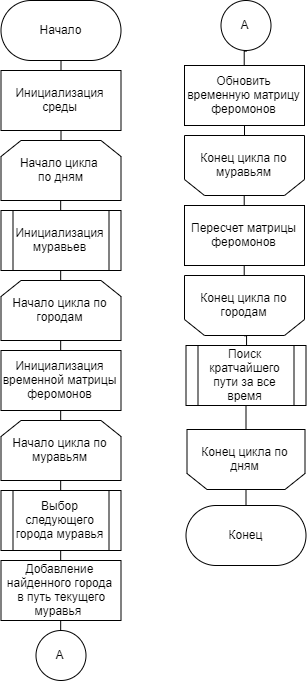
\includegraphics[scale = 0.7]{Ant.png}}
		\caption{Схема алгоритма решения задачи коммивояжера.}
		\label{fig:ant}
	\end{figure}
	
	\subsection{Вывод}
	\hspace*{5mm} В данном разделе были рассмотрены требования к программе и схемы этих алгоритмов. 


\newpage
\section{Технологическая часть}

	\hspace*{5mm} В данном разделе будут рассмотрены требования к программному обеспечению, средства реализации и представлен листинг кода.
	\subsection{Требования к программному обеспечению}
		\begin{enumerate}
		\item программа должна корректно находить кратчайший путь;
		\item программа должна обеспечить возможность замера времени работы алгоритма. 
	\end{enumerate}
	На Рисунке 2 показана представлена IDEF0-диаграмма описывающая функциональную схему алгоритма Муравья.
	\begin{figure}[h]
		\center{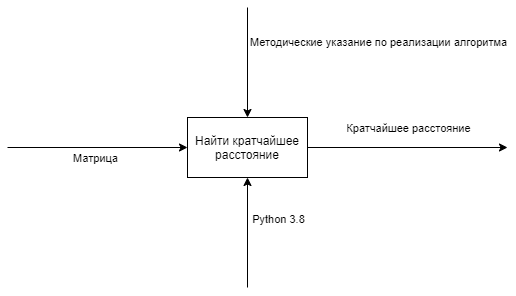
\includegraphics[scale = 0.7]{a.png}}
		\caption{IDEF0-диаграмма, описывающую функциональную схему алгоритма Мурвья.}
		\label{fig:ant}
	\end{figure}
	\subsection{Средства реализации}
	\hspace*{5mm} В данной работе используется язык программирования Python, за высокую скорость выполнения программ и широкий выбор инструментов для параллельных вычислений.\cite{doc} Проект выполнен в среде разработки Visual Studio Code. Многопоточное программирование было реализовано с помощью ThreadPoolExecutor.\cite{paral} 
	\clearpage
	\newpage 
	\subsection{Листинг кода}
	В данном пункте представлен листинг кода.
	\definecolor{codegreen}{rgb}{0,0.6,0}
	\definecolor{codegray}{rgb}{0.5,0.5,0.5}
	\definecolor{codepurple}{rgb}{0.58,0,0.82}
	\definecolor{backcolour}{rgb}{0.95,0.95,0.92}

	\lstdefinestyle{mystyle}{
		backgroundcolor=\color{backcolour},   
		commentstyle=\color{codegreen},
		keywordstyle=\color{magenta},
		numberstyle=\tiny\color{codegray},
		stringstyle=\color{codepurple},
		basicstyle=\ttfamily\footnotesize,
		breakatwhitespace=false,         
		breaklines=false,                 
		captionpos=b,                    
		keepspaces=true,                 
		numbers=left,                    
		numbersep=5pt,                  
		showspaces=false,                
		showstringspaces=false,
		showtabs=false,                  
		tabsize=2
	}

	\lstset{style=mystyle}

	\hspace*{-7mm} На листинге 1 представлен код муравьиного алгоритма.
	\begin{lstlisting}[language=Python, caption = Муравьиный алгоритм]
def best_way(m, e, matr, t_max, alpha, beta, ro, q):
	nue = 1 / matr  
	
	teta = np.random.sample((m, m))  
	T_min = None  
	L_min = None   
	
	t = 0  
	
	while t < t_max:
		teta_k = np.zeros((m, m)) 
		for k in range(m):  
			Tk = [k] 
			Lk = 0 
			i = k   
	
			while len(Tk) != m:
				J = [r for r in range(m)]  
				for c in Tk: 
					J.remove(c)
	
				P = [0 for a in J]  
				for j in J:
	
					if matr[i][j] != 0: 
						buf = sum((teta[i][l] ** alpha) * (nue[i][l] ** beta) for l in J)
						P[J.index(j)] = (teta[i][j] ** alpha) * (nue[i][j] ** beta) / buf
					else:
						P[J.index(j)] = 0
	
				Pmax = max(P)
				if Pmax == 0:
					break
	
				index = P.index(Pmax) 
				Tk.append(J[index])   
				Lk += matr[i][J[index]]  
				i = J.pop(index)  
	
			if L_min is None or (Lk + matr[Tk[0]][Tk[-1]]) < L_min: 
				L_min = Lk + matr[Tk[0]][Tk[-1]]                   
				T_min = Tk
	
			for g in range(len(Tk) - 1):  
				a = Tk[g]
				b = Tk[g + 1]
				teta_k[a][b] += q / Lk
	
		teta_e = (e * q / L_min) if L_min else 0   
		teta = (1 - ro) * teta + teta_k + teta_e     
		t += 1
	
	return T_min, L_min
	\end{lstlisting}
	
	\subsection{Вывод}
	\hspace*{5mm} В данном разделе была представлена структура ПО и листинги кода программы. 
	


\newpage
\section{Исследовательская часть }

	\hspace*{5mm} В данном разделе будет проведен эксперимент и сравнительный анализ.
	\subsection{Системные характеристики}
	Характеристики компьютера на котором проводился замер времени сортировки массива:
	\begin{enumerate}
		\item операционная система - Windows 10;
		\item процессор - Intel(R) Core(TM) i7-10510U CPU @1.80GHz 2.30GHz;
		\item оперативная память - 16 ГБ;
		\item количество ядер - 4;
		\item количество логических процессов - 8.
	\end{enumerate}
	\subsection{Постановка эксперимента}
	В рамках данного проекта были проведены эксперименты, описанные ниже:
	\begin{enumerate}
		\item сравнение и анализ времени работы алгоритма при разных входных данных.
	\end{enumerate}
	\subsection{Сравнительный анализ на основе замеров времени работы программы}
	Был проведен замер времени работ.
	\\ \hspace*{5mm} В Таблице 1 показаны результаты замера времени при разных входных параметрах. Число муравьев варировалось от 100 до 500. Количество потоков было равно 10. Ниже приведена полученная таблица:
	\clearpage
	\newpage
	\begin{table}[h]
		\centering
		\caption{Результаты временного замера при разных входных параметрах.\\}
		\begin{tabular}{ | c | c | c | c | c | c | c |}
			\hline
			$N$ & $t$ & $Q$ & $e$ & $\alpha$ & $\beta$ & $\rho$  \\ \hline
			100 & 0.03125 & 5 & 0 & 1 & 1 & 0.6 \\ \hline
			100 & 0.14062 & 50 & 0 & 2 & 3 & 0.3 \\ \hline
			100 & 0.12500 & 5 & 0 & 3 & 3 & 0.3 \\ \hline
			100 & 0.12500 & 25 & 3 & 2 & 2 & 0.2 \\ \hline
			100 & 0.10938 & 25 & 1 & 2 & 2 & 0.1 \\ \hline
			200 & 0.20312 & 25 & 3 & 1 & 3 & 0.7 \\ \hline
			200 & 0.23438 & 25 & 0 & 3 & 1 & 0.1 \\ \hline
			200 & 0.21875 & 25 & 2 & 1 & 3 & 0.4 \\ \hline
			200 & 0.31250 & 25 & 0 & 1 & 3 & 0.5 \\ \hline
			200 & 0.26562 & 25 & 2 & 1 & 1 & 0.2 \\ \hline
			300 & 0.53125 & 50 & 0 & 2 & 2 & 0.3 \\ \hline
			300 & 0.51562 & 25 & 1 & 2 & 3 & 0.6 \\ \hline
			300 & 0.53125 & 5 & 3 & 1 & 3 & 0.3 \\ \hline
			300 & 0.37500 & 50 & 0 & 1 & 3 & 0.2 \\ \hline
			300 & 0.43750 & 50 & 0 & 1 & 3 & 0.5 \\ \hline
			400 & 0.56250 & 25 & 0 & 1 & 3 & 0.2 \\ \hline
			400 & 0.60938 & 5 & 3 & 3 & 2 & 0.2 \\ \hline
			400 & 0.75000 & 50 & 0 & 1 & 2 & 0.1 \\ \hline
			400 & 0.56250 & 50 & 3 & 3 & 3 & 0.4 \\ \hline
			400 & 0.57812 & 50 & 2 & 3 & 2 & 0.7 \\ \hline
			500 & 1.01562 & 5 & 0 & 1 & 1 & 0.7 \\ \hline
			500 & 0.90625 & 5 & 0 & 1 & 1 & 0.5 \\ \hline
			500 & 0.95312 & 50 & 2 & 3 & 3 & 0.7 \\ \hline
			500 & 1.06250 & 25 & 0 & 1 & 3 & 0.2 \\ \hline
			500 & 0.78125 & 25 & 0 & 1 & 2 & 0.6 \\ \hline
			
		\end{tabular}
	\end{table}
	\clearpage
	\newpage
	В результате проведенных испытаний было установлено, что:\\
	\begin{enumerate}
		\item Судя по проведенным выше дааным, самое точное приближение не всегда является самым выгодным. Проверим это утверждение на тестовом случае с фиксацией всех параметров, кроме $Q$. Проведем несколько тестовых запусков с $Q \in [1, 50]; t = 200; m = 5, e = 1; \rho = 0.3; \alpha = 1; \beta = 1.$ На Рисунке 3 показаны результаты этого эскперимента:\\
		\begin{figure}[h!]
			\center{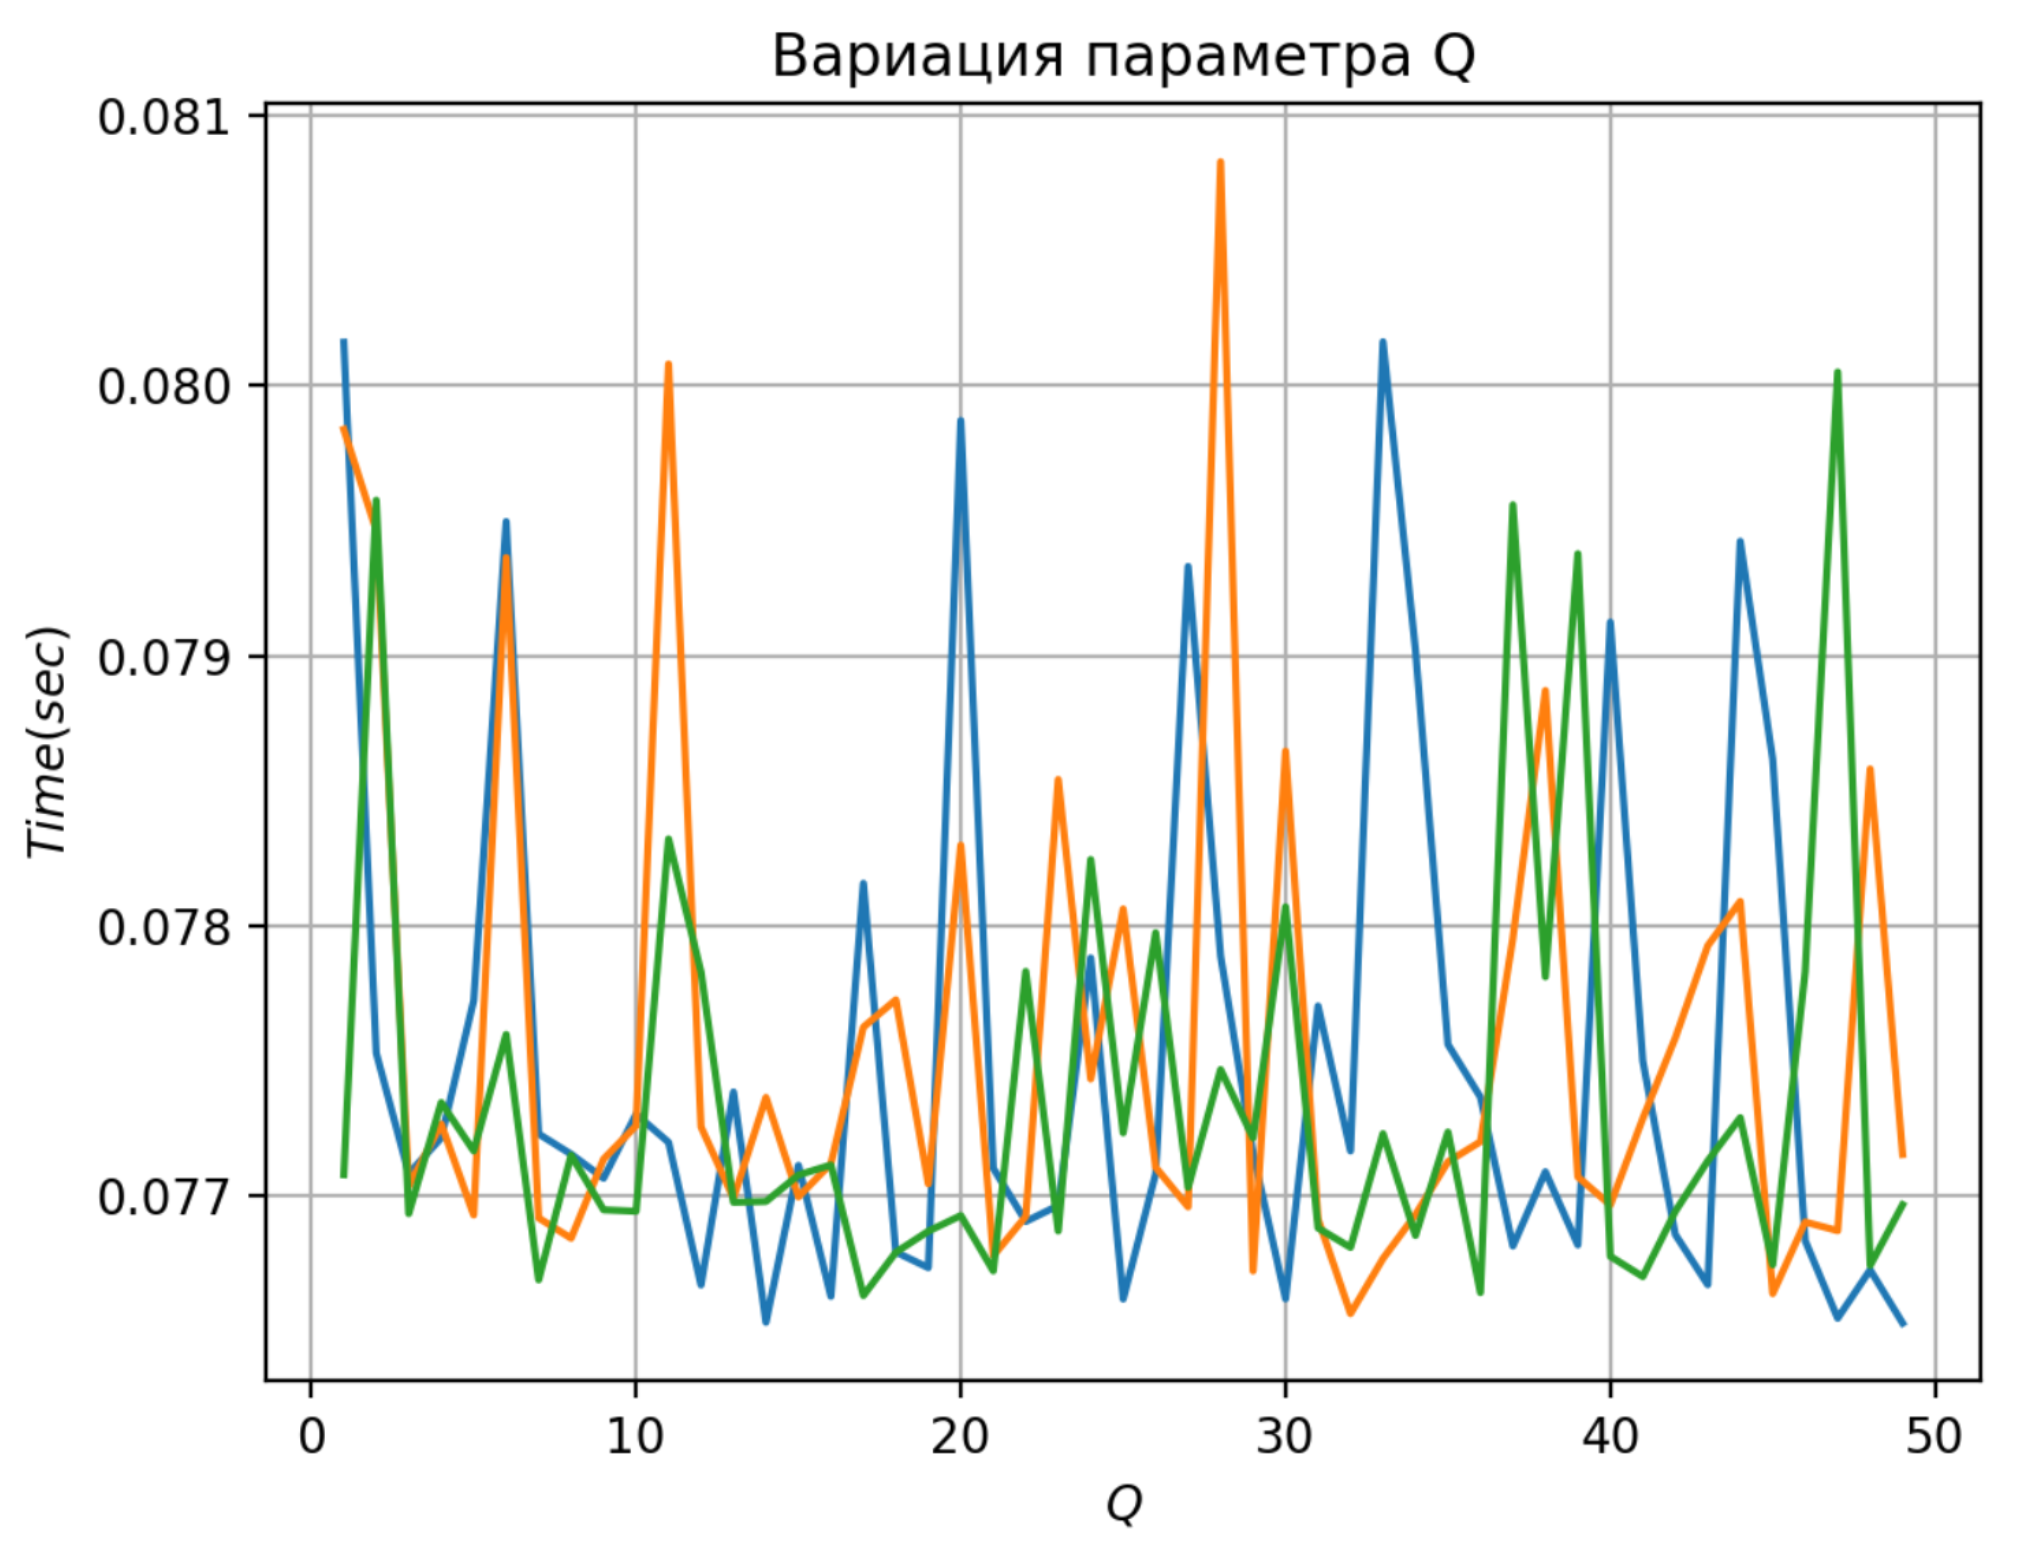
\includegraphics[scale = 0.6]{chart1}}
			\caption{Эскперимент с $Q \in [1, 50]; t = 200; m = 5, e = 1; \rho = 0.3; \alpha = 1; \beta = 1.$}
		\end{figure}
		Как видим результат варьируется от случая к случаю.
		\item Наличие элитных муравьев улучшает сходимость. Однако в оптимальных наборах их количество сильно связано с коэффициентами $\alpha и \beta$, отвечающими за мощность феромонного запаха и за желание муравья передвигаться по этому пути соответственнно. Объяснить это можно так: так и тот, и другой аспект алгоритма усиливает феромоновую дорожку, то их подбор должен быть сбалансирован, так как возможно "зависание" на локальных эсктремумах. На Рисунке 4 показаны графики вариации компонентов $e, \alpha, \beta, \rho$:
		\clearpage
		\newpage
		\begin{figure}[h]
			\center{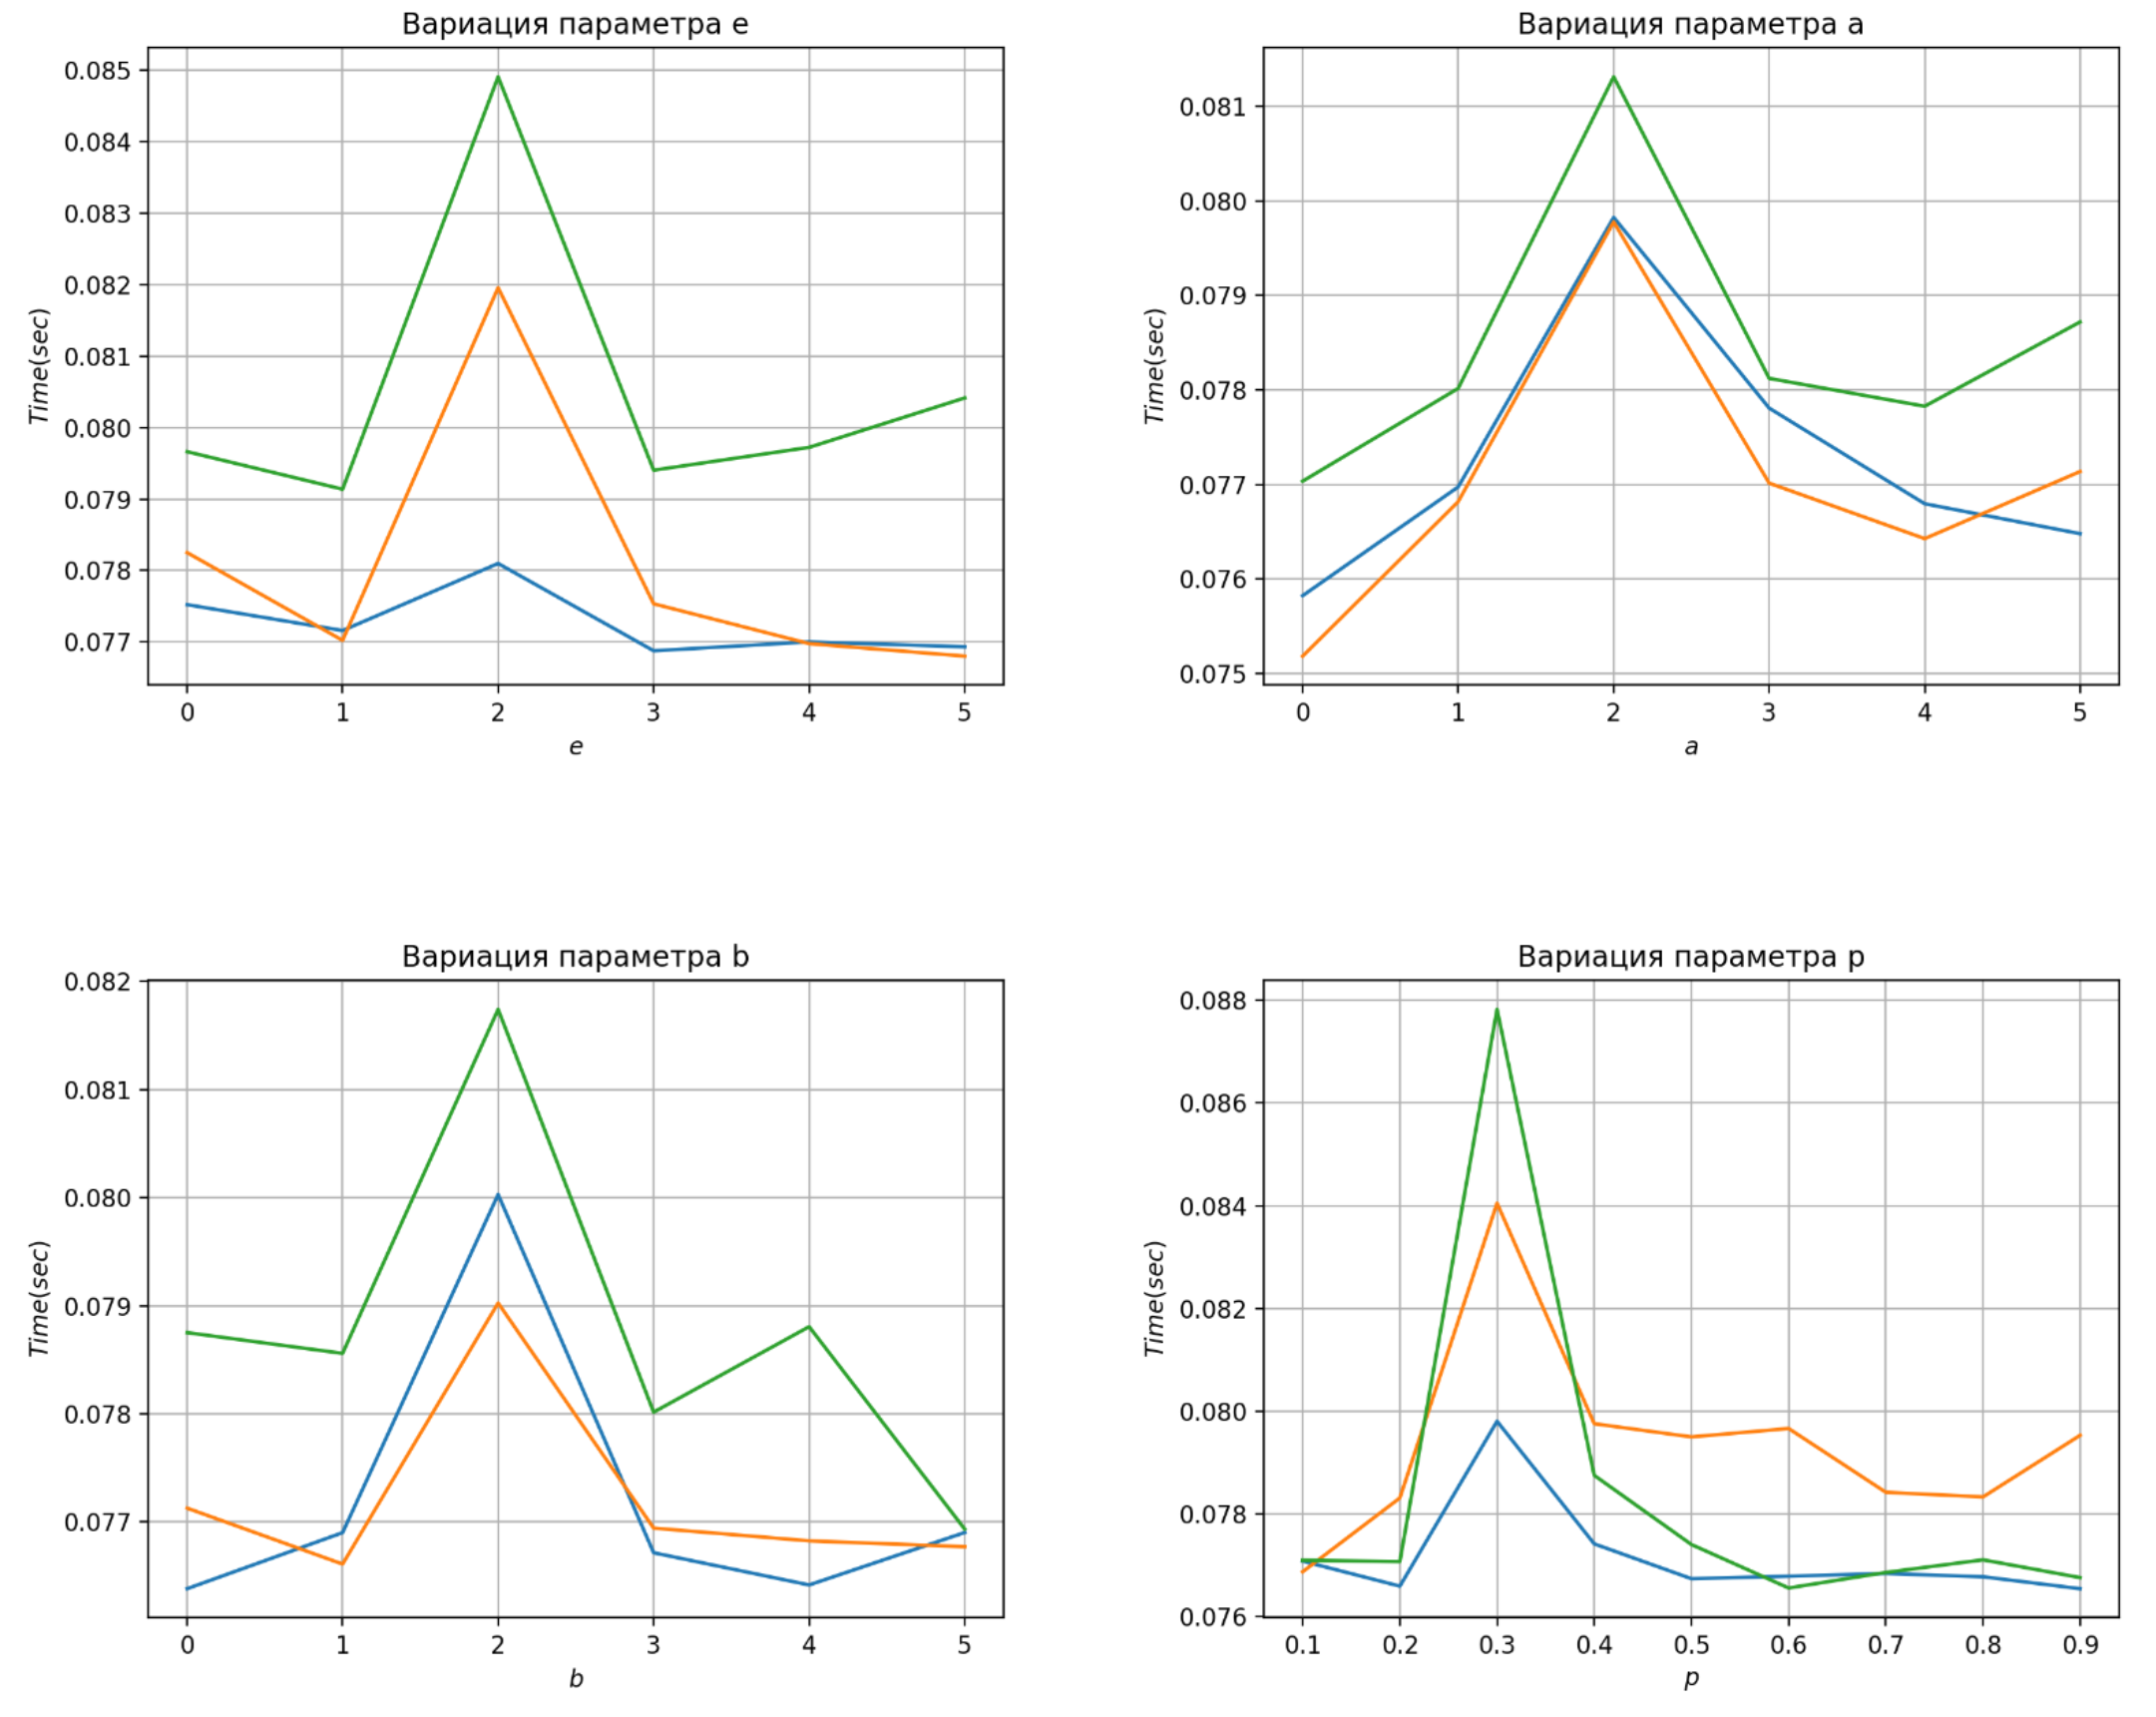
\includegraphics[scale = 0.6]{chart2}}
			\caption{Эскперимент с вариацией комнонетов $e, \alpha, \beta, \rho$.}
		\end{figure}
		\item На графиках видны "нежелательные" значения параметров: $e = 2, \alpha = 2, \beta = 2, \rho = 0.3$. Это может быть обусловлено математическими особенностями алгоритма.
	\end{enumerate}  
	
	\subsection{Вывод}
	\hspace*{5mm} По проведенному анализу  эксперимента можно сделать вывод, что самое точное приближение не всегда является самым выгодным. Наличие элитных муравьев улучшает сходимость. Однако в оптимальных наборах их количество сильно связано с коэффициентами $\alpha и \beta$, отвечающими за мощность феромонного запаха и за желание муравья передвигаться по этому пути соответственнно. Объяснить это можно так: так и тот, и другой аспект алгоритма усиливает феромоновую дорожку, то их подбор должен быть сбалансирован, так как возможно "зависание" на локальных эсктремумах.



	\newpage
	\section*{Заключение}
	\hspace*{5mm} В рамках данной работы успешно изучены основы муравьиного алгоритма. Применен метод асинхронного программирования. Проведен сравнительный анализ при разных параметрах. Подтверждены экспериментально "нежелательные" параметры значения параметро. Дано описание и обоснование полученных результатов.   


\clearpage
\newpage

\printbibliography

\end{document}